\section{Methodology}

In this section, we will describe how we collected the data, we will present an analysis of the data, and then lead into the discussion of the machine learning models used.

\subsection{Collection}

Our collection began with the development of an Android application that connected to a Microsoft Band smartwatch and collected data from all of its available sensors. This development led to the general Android-based sensor gateway discussed in the previous section. Next, we developed a general procedure for our volunteers to follow during the collection of data. Our volunteers were eager to freely contribute the anonymous data used in this paper. The system collected the data into a .csv file on the Android smartphone and was also transmitted to a central MySQL server.

The Android platform was version 5.0 (kernel 3.4.0-4432708) running on a Samsung S5 smartphone. The Microsoft Band was Build Version 10.2.2818.0 09 R. Samples of the sensor data were collected every three seconds, based on the update speed of the Band's heart rate sensor. For every sample, the most recent sensor value was used for every sensor if available, else it would use the last updated value; or in the case of the accelerometer and gyroscope sensors, the last three values were averaged with linear weighting (the most recent having the most importance). There may be a better weighting, but this weighting was suitable for our purposes.

We designed a simple, two-hour procedure for the collection of the data. First, we established some necessary information about the subject to estimate the amount of alcohol necessary to reach 0.08 BAC in a 1.5 hour period using the Widmark equation (1). The particular formulation of it we used is the following: \begin{equation}
SD =  BW \cdot Wt \cdot (EBAC + (MR \cdot DP)) \cdot 0.4690
\end{equation} where $SD$ is the number of standard drinks (10 grams ethanol), $BW$ is the body water contant (0.58 for men and 0.49 for women), Wt is the body weight in lbs, EBAC is the estimated BAC, MR is the metabolism rate (0.17 for women and 0.18 for men), DP is the drinking period in hours, and  $0.4690 = 0.4536 \div (0.806 \cdot 1.2)$, a combination of two constants from the equation and a converstion from kg to lbs \cite{Andersson:2009}\cite{Wiki:BAC}. This amount was used to estimate the number of standard drinks to be consumed over the set time period, distributed over equal intervals. During this process, at every 25 minutes we took a measurement of the BAC using a BACtrack Trace\textsuperscript{TM} Pro breathalyzer. This measurement interval was determined by the cooldown rate of the breathalyzer. The activity chosen for the volunteers to engage in was a card or board game of their choice. Drinking stopped before 1.5 hours while collection and BAC measurement continued for another 30-45 minutes.

\subsection{Data Analysis}

The Microsoft Band we used has an assortment of interesting physical and virtual sensors that we can look at, including: an accelerometer, a gyroscope, distance, heart rate, pedometer, skin temperature, and ultraviolet level. With the sample size of five volunteers and a controlled setting for the experiments, some will not be as useful for this study: distance, pedometer, and ultraviolet level. In fact, their usefulness may be limited even with larger datasets. 

We begin our analysis with the heart rate (HR) by normalizing the heart rates and BACs per subject. This way we can plot and compare the HR values over the BAC and see if there are any obvious patterns. Doing this we get the plots shown in Figure \ref{fig:heart_rate_facet}.

\begin{figure}
	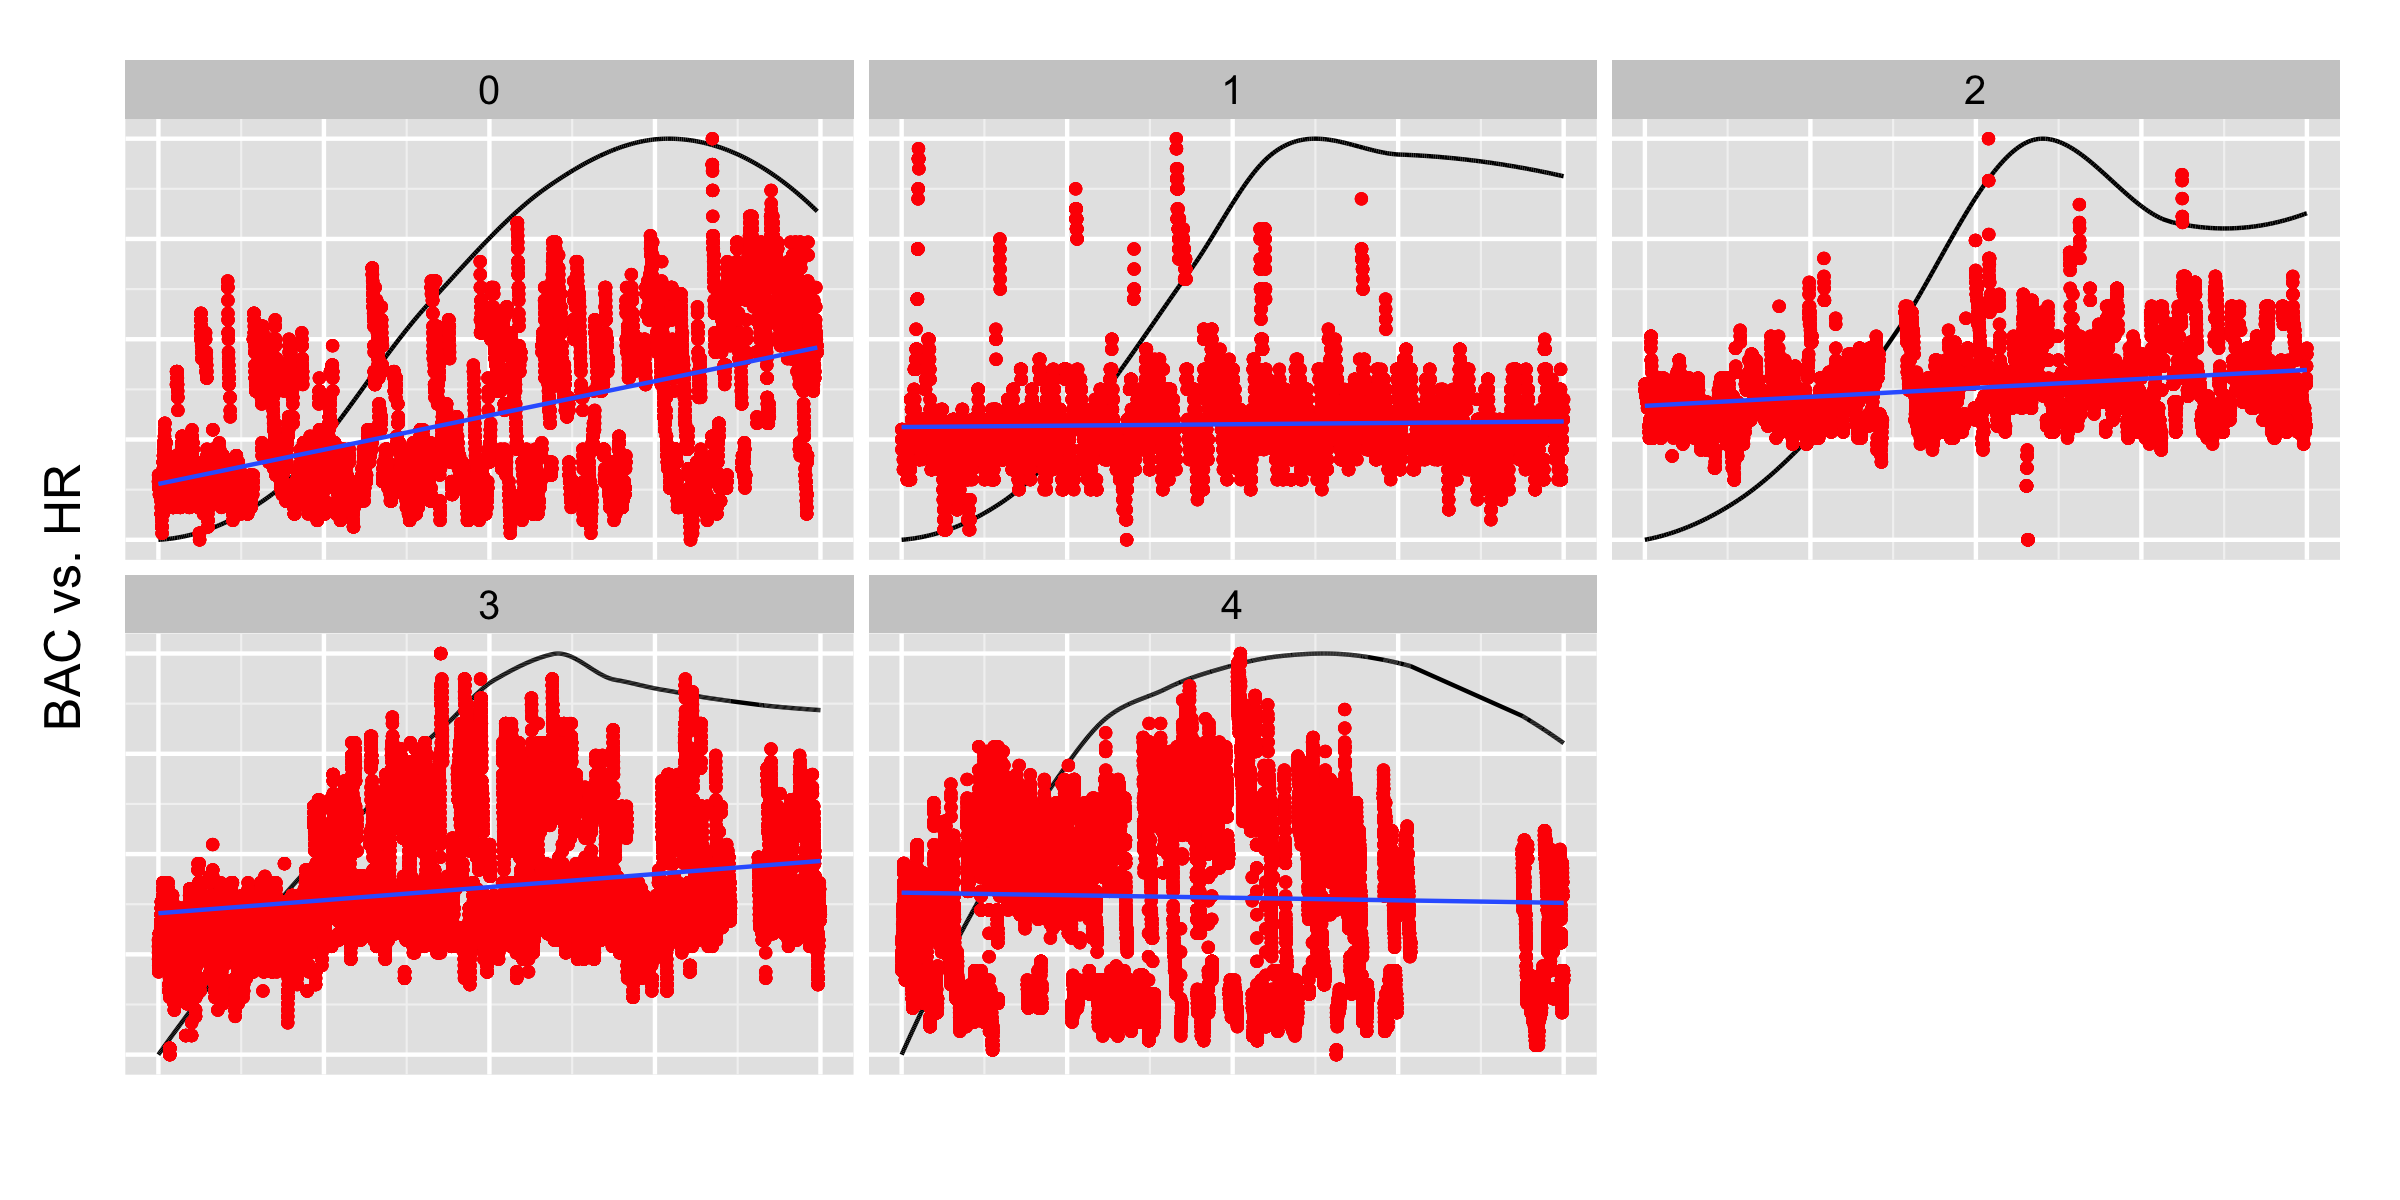
\includegraphics[width=1.0\textwidth]{../figs/heart_rates}
	\caption{Heart Rate and BAC per subject (normalized).}
	\label{fig:heart_rate_facet}
\end{figure}

The heart rate increases over time for three of the subjects (0, 2, 3) at different rates, decreases for one (4), and stays level for one (1). These observations are consistent with data in \cite{Assaad:2006}; a study where the authors relate low and high HR responses to behavioral traits. Interestingly, most of the subjects seem to show two patterns of HR activity. One is the baseline HR activity, and another is an excitied HR activity that seems to have better correlation with BAC. This is most clearly seen in the plot for subject 0, shown in Figure \ref{fig:heart_rate_split}. \begin{figure}
	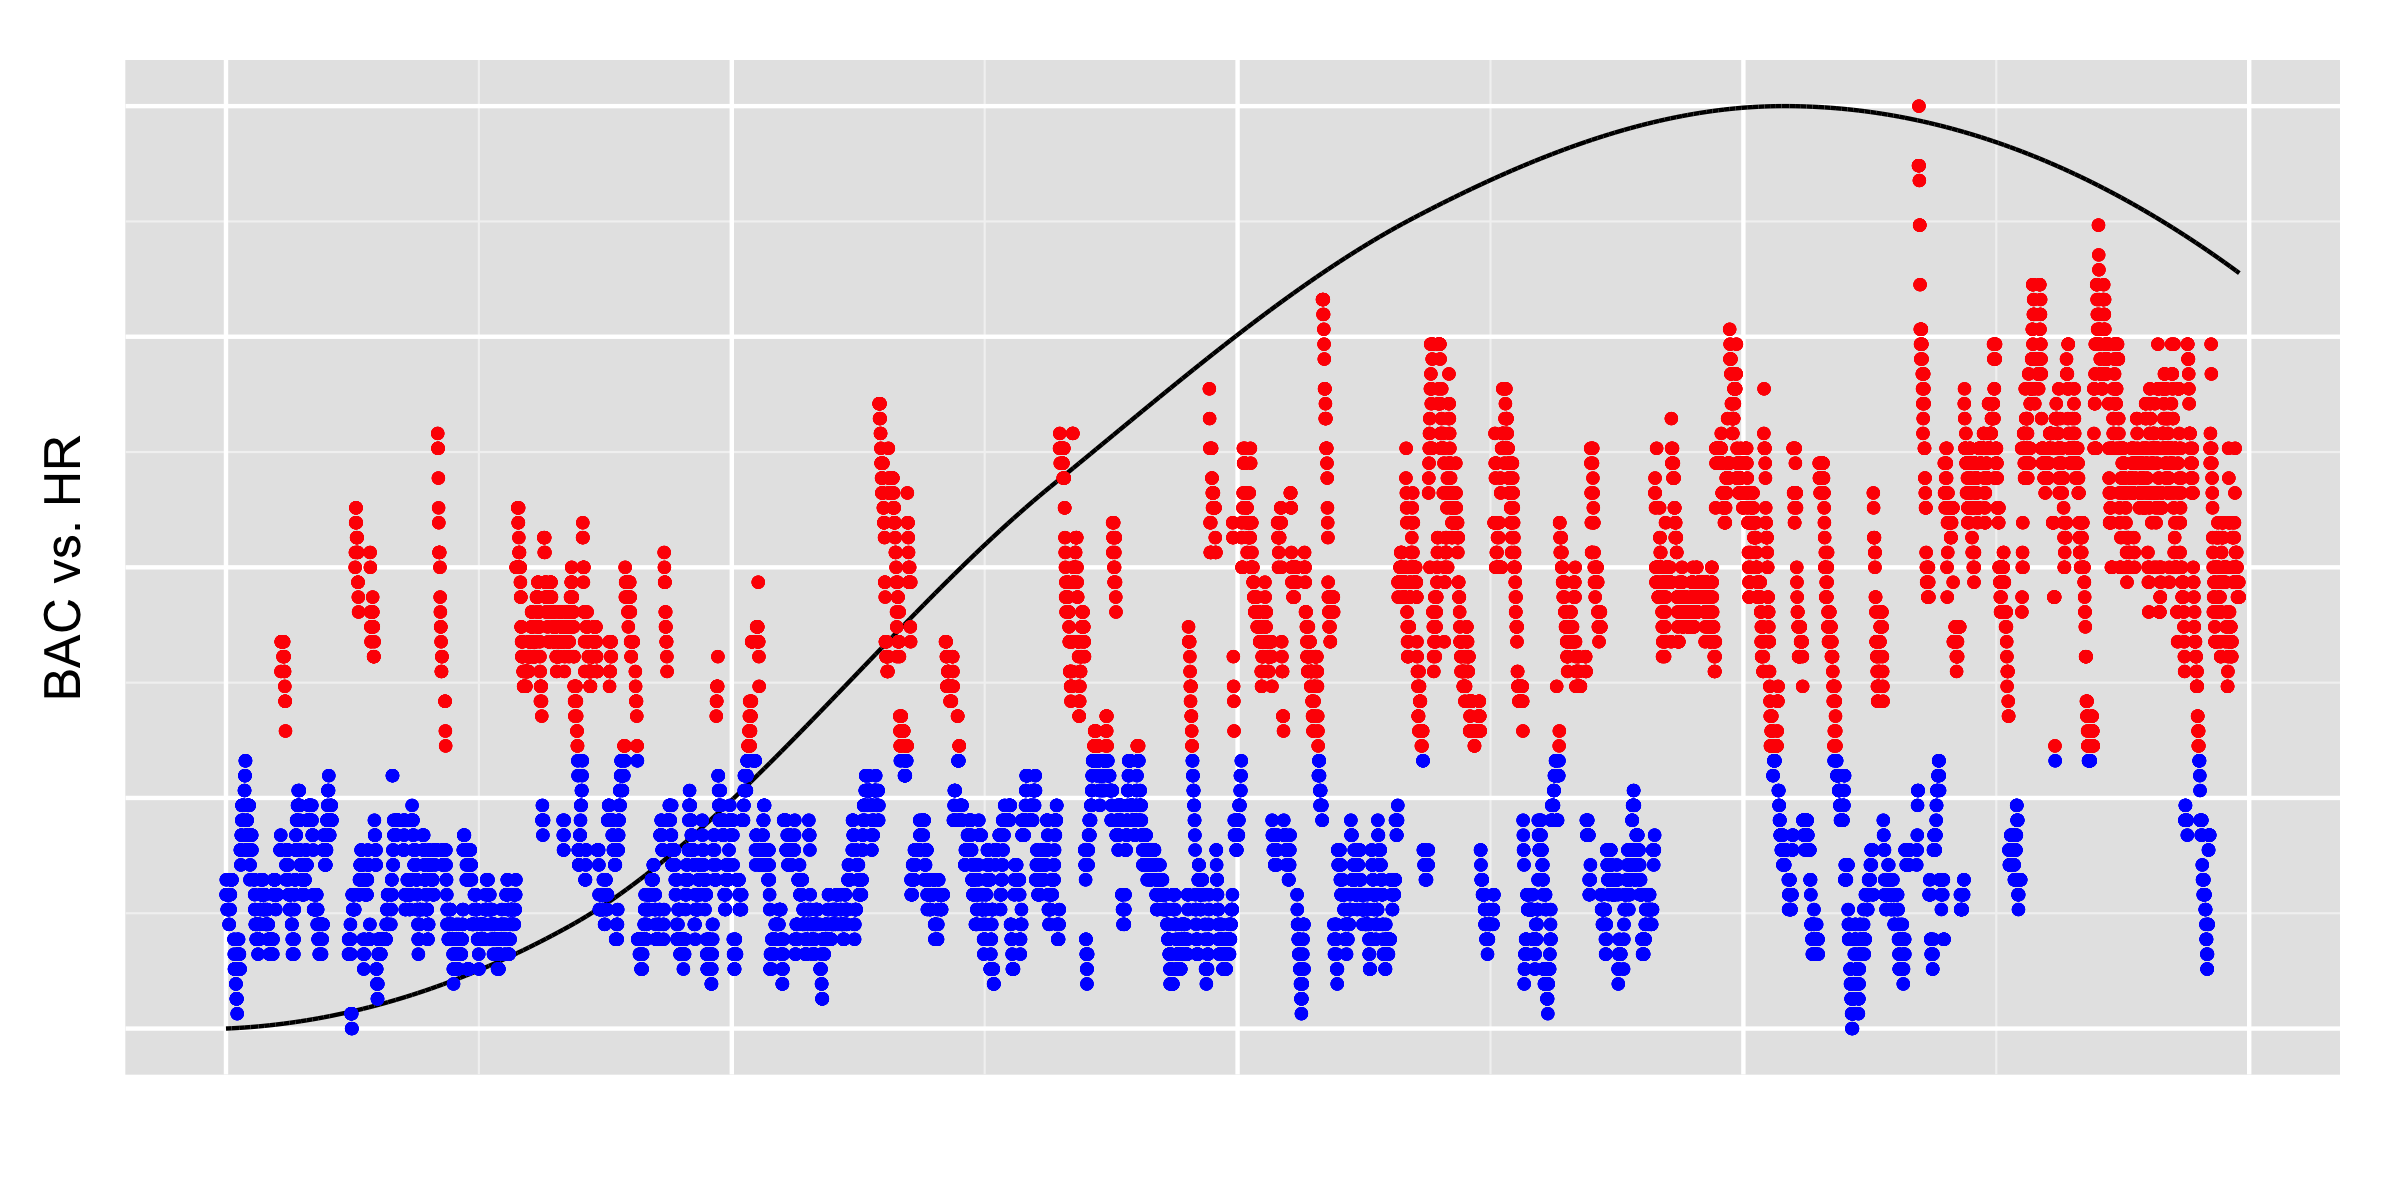
\includegraphics[width=1.0\textwidth]{../figs/heart_rate_split}
	\caption{Heart rate split into baseline and excited states.}
	\label{fig:heart_rate_split}
\end{figure}It's not a consistent pattern, however. Subject 1 had a very level heart rate with spikes at the regular drinking intervals, and subject 2 had relatively little variance throughout. Overall, it seems that experiencing excitement while intoxicated results in a more exaggerated HR response than while sober. This may be useful information for determining drunkenness.

Next, we plotted the normalized skin temperature over time on top of the normalized BAC values; this is shown in Figure \ref{fig:skin_temperatures}. \begin{figure}
	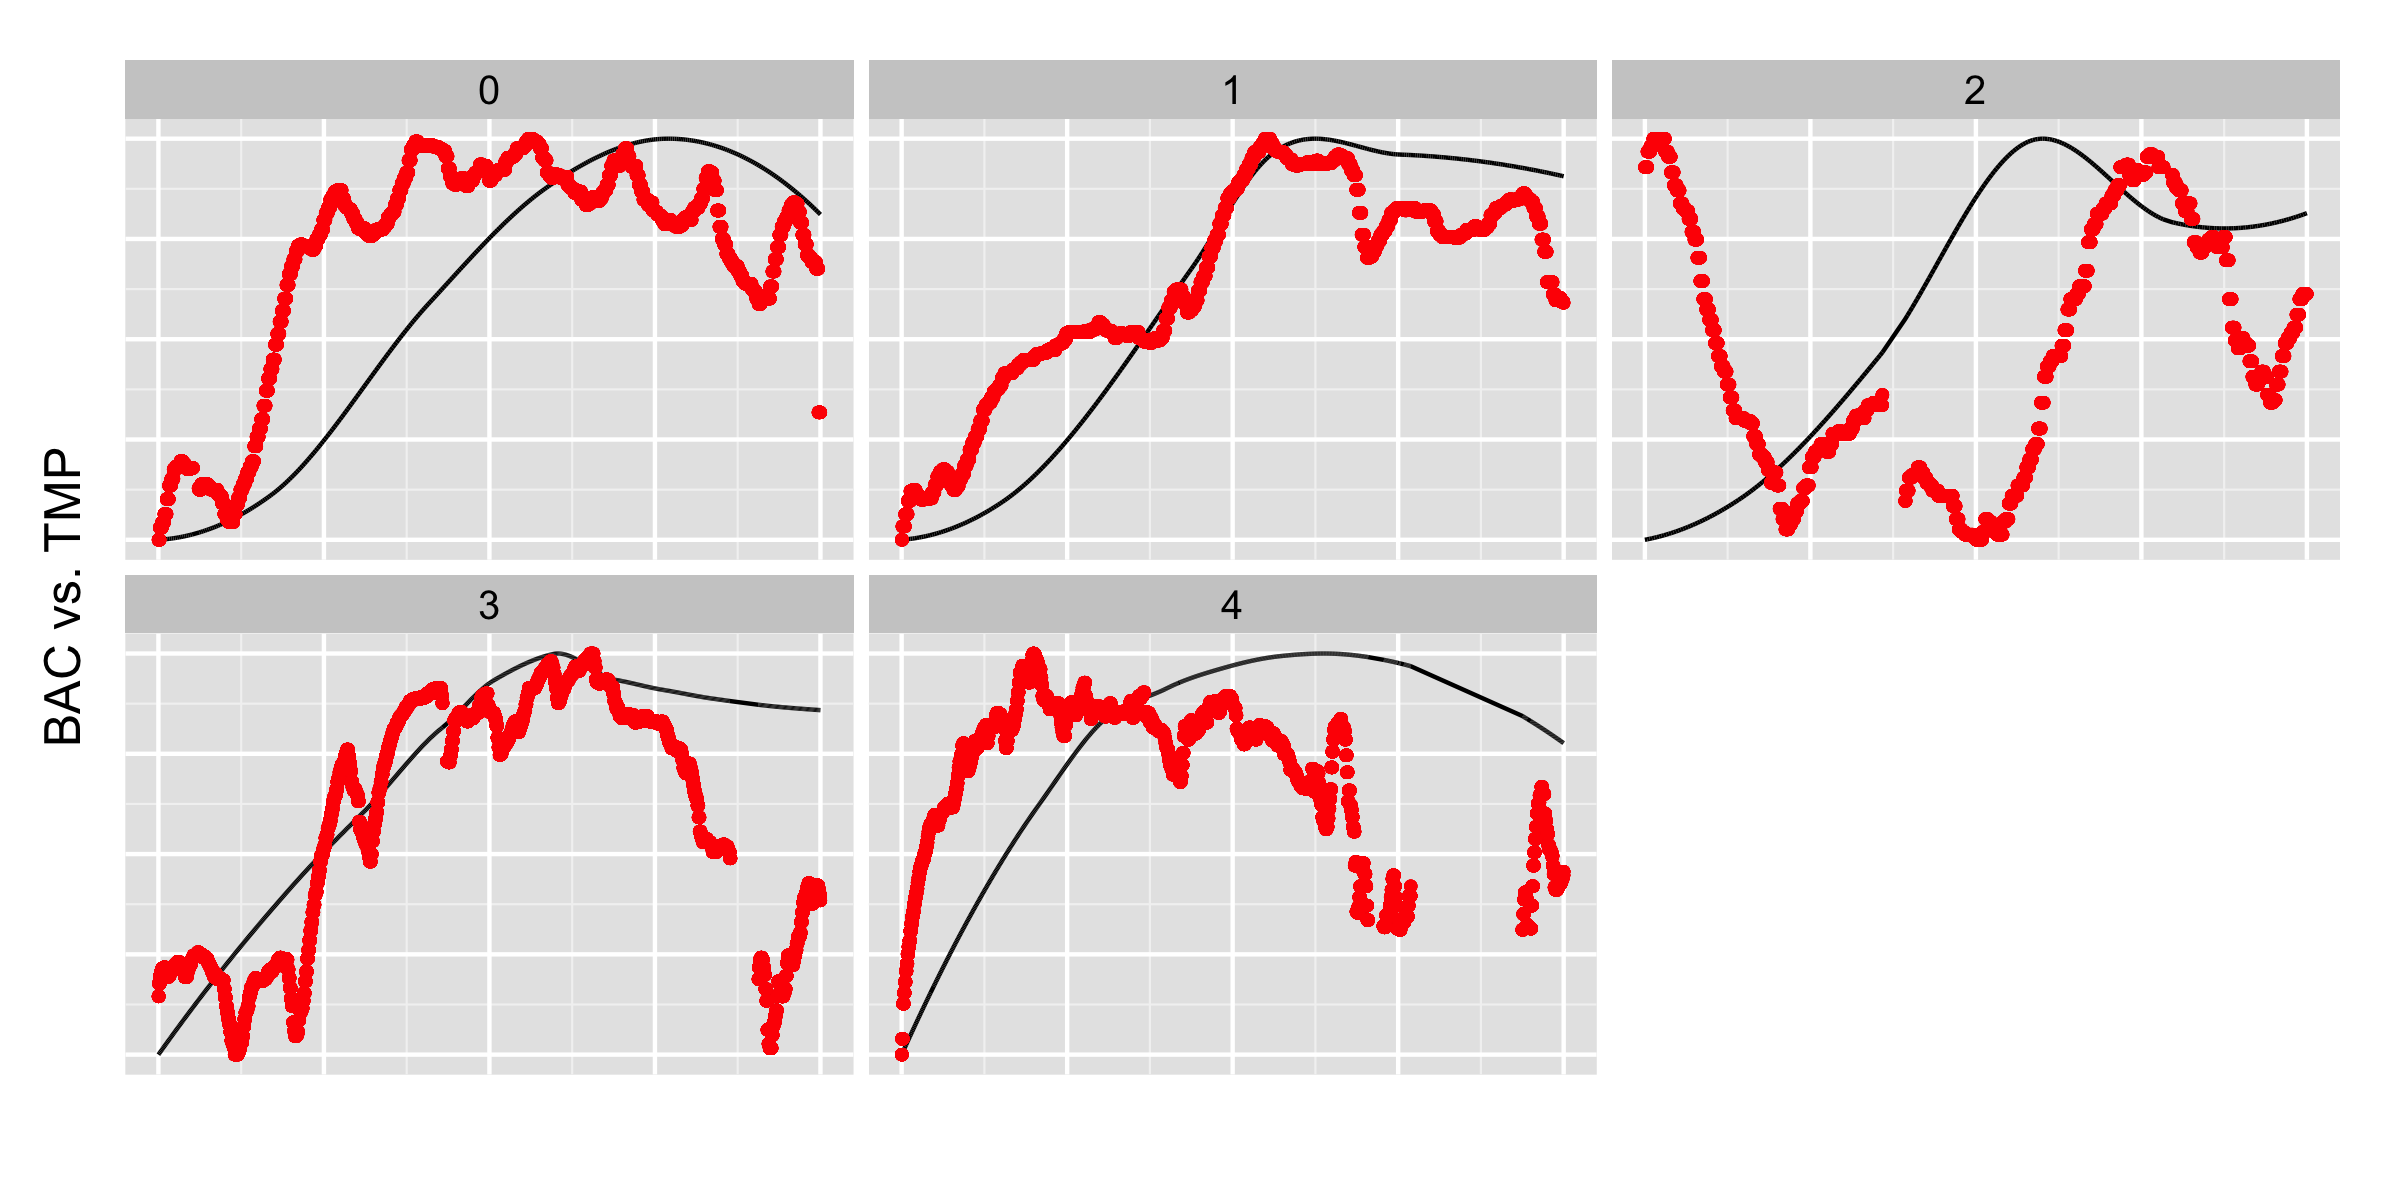
\includegraphics[width=1.0\textwidth]{../figs/skin_temperatures}
	\caption{Skin Temperature and BAC per subject (normalized).}
	\label{fig:skin_temperatures}
\end{figure}Visually, we see that the correlation of skin temperature and BAC is highly significant. This is because of the well known vasodilation effect of alcohol causing warm blood to come near the surface of the skin \cite{Dekker:1999}. It is also known that with a high enough level of intoxication it behaves as a vasoconstrictor and drops skin temperature, which we see with subjects 4 and 5 who had reached the highest BAC of the group. Subject 2 had a rapid decrease in temperature at the beginning (we may have started collection too soon before the smartwatch sensor adjusted to his skin temperature), it may be appropriate to discard this portion.

The movement sensors (accelerometer and gyroscope) were not too interesting visually or statistically. They might have some hidden patterns that contribute to the performance of a modeling technique. We think it's usefulness will be increased if we can use it first to predict whether a user is taking a drink, then provide a time-based aggregate of the estimated number of drinks as a feature in our model to determine drunkenness.

\subsection{Features Setup}

Skin temperature and heart rate will have different ranges of values unique to each subject, so per-subject normalization must be performed to put them on the same scale. A simple unity-based normalization (min-max) is used to put the feature values in the range 0 to 1. No transformations are applied to the movement data.

\subsection{Models and Tools}

We will be taking a look at BAC prediction as both a classification and regression problem. As a classification problem, we will threshold the BAC values at a point where we may want to warn the user. This allows the data to be used as a binary classification problem. For this we will use logistic regression and SVM. 

As a regression problem, we will be attempting to predict the observed BAC directly. To do this, we will use linear regression and artificial neural networks (ANN). Using a regression approach, this will allow a user to select their own threshold rather than the threshold determined in a classification model. We may however want the threshold to be fixed.

All work will be performed in R version 3.2.1 using the additional 'nnet' and 'kernlab' packages. Any necessary additional information will be provided in the evaluation section.